\section{背景}
近年,コンテンツをノード,コンテンツ間の関係性をエッジとみなしたグラフ表現・解析を行うことへの注目が高まっている.
Social Network Service の友人関係や,World Wide Web の参照関係などがグラフとして表現される代表例であり,年々これらの
グラフサイズは巨大化している.
\cite{ching2015one}では,2015 年時点で Facebook グラフのエッジ数は 1 兆を上回ると報告されており, 
今後もグラフサイズの巨大化は継続していくと予想される.
また,現在は単一主体によるグラフの集中管理が主流であり,コンテンツ間の関係性を定義するのはグラフの管理者である.
このような管理形態では,様々な主体が自由にコンテンツ間の関係性を見出し,その価値を流通させることは困難である.
そこで,巨大化し続けるグラフに対してスケーラビリティを確保しつつ,様々な主体が自由にコンテンツ間の関係性を定義可能なグラフ管理形態
として,自律分散グラフ管理を考える.

自律分散グラフ管理環境では,様々な主体が部分的にグラフを管理し,部分グラフの重ね合わせとして全体グラフが構成される.
各部分グラフの管理者は,管理下のコンテンツに対して自由に関係性を定義し,エッジとして保持する.
また,全体グラフを集中管理する必要はないので,グラフサイズに対するスケーラビリティも確保される.
自律分散グラフ管理を適用したシステムの例として Catalogue \cite{catalogue}などが存在する.

一般に,分散管理された巨大グラフを全取得するコストは大きい.
そこで,自律分散グラフ管理環境では PageRank (PR) \cite{page1999pagerank} や Personalized PageRank (PPR) \cite{page1999pagerank} などの
グラフ演算を実行する場合,着目ノードからランダムウォーク (RW) を実行し,演算対象の部分グラフを取得する.
RW によるグラフ取得では着目ノードを始点として,確率 1-α で隣接ノード群からランダムに選択したノードへ,確率 α で始点へ移動するという操作を繰り返し,
全体の軌跡を部分グラフとして取得する.
ID 10 のノードを始点とした場合の RW によるグラフ取得の例を図\ref{RW_graph} に示す.
\begin{figure}[t]
  \centering
  %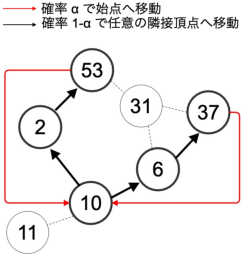
\includegraphics[width=\linewidth]{./figure/rw_graph.pdf}
  %\includegraphics[scale=1.0]{./figure/RW_graph.pdf}
  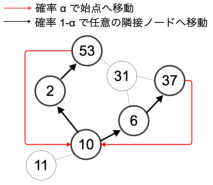
\includegraphics[scale=1.8]{./figure/rw_graph_get.pdf}
  \caption{ランダムウォークによるグラフ取得}
  \label{RW_graph}
\end{figure}
なお,RW による取得の特徴として全体グラフの構造を維持しながら部分グラフの取得が可能という点が挙げられる.
PR や PPR などのグラフ演算実行時にはメモリへの不規則なアクセスによるキャッシュミスが多発する.
\cite{wei2016speedup,zhang2017making} では,演算時間の約 70 \% がキャッシュミスに伴う
メインメモリへのアクセス時間によるものと報告されており,キャッシュミスは演算速度低下を引き起こす重大な要因の1つである.
そこで,グラフ演算時のキャッシュミスを減少させるために,
前処理として各ノードに割り振られた ID を適切に再配置する手法が提案されている \cite{wei2016speedup,zhang2017making,balaji2018graph,arai2016rabbit,lakhotia2017recall,faldu2019closer}.
ノード ID を再配置する例を図\ref{reordering_intro}に示す.
\begin{figure}[t]
  \centering
  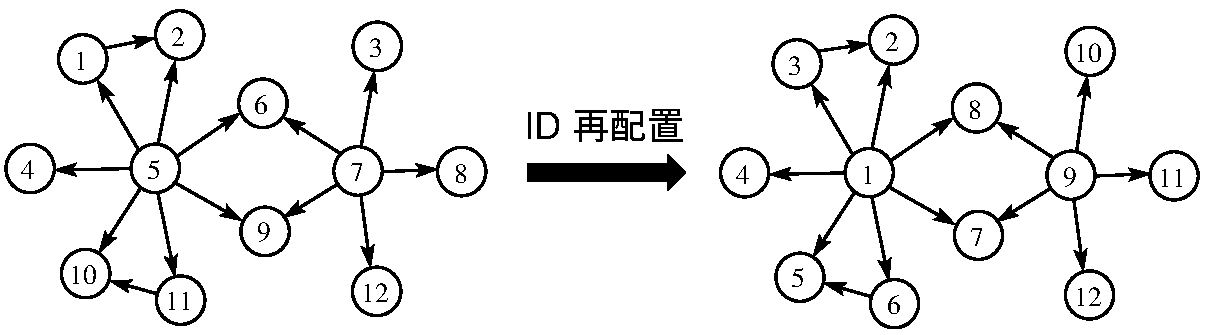
\includegraphics[width=\linewidth]{./figure/reordering_intro.pdf}
  \caption{ノード ID 再配置の例}
  \label{reordering_intro}
\end{figure}
既存のノード ID 再配置手法はグラフの全体構造が把握可能という前提のもとで議論がされている.
しかし,グラフ取得が完了するまで全グラフが手元にない状況で既存の再配置手法を適用するにはグラフ取得の完了を待つ必要がある.
取得完了を待つに伴い,再配置実行前のグラフ構造を保持するメモリ領域が必要となったり,グラフ取得を待つだけの無駄な待ち時間が発生するなど
空間・時間コストが増加する.
そこで,グラフを取得しながらノード ID を再配置することで,時間・空間コストを削減する手法が必要となる.
既存の再配置手法ではグラフの全体構造が把握可能という前提のもと,演算時のアクセス局所性のみ考慮しているが,グラフを取得しながら再配置を行う場合,アクセス局所性に加え,ID の連続性も考慮する必要がある.

本研究では,グラフを取得しながらノード ID を再配置する手法として,連続性・アクセス局所性をそれぞれ意識した Sequential, DBG Early Estimation (DBG-EE) を提案する.
そして,Sequential, DBG-EE の効果を演算時間の減少率から明らかにする.また,グラフ取得の完了を待たないことによる空間・時間コストの変化を 
ID 再配置に必要なメモリ使用量及びグラフ取得と演算の合計時間から明らかにする.

\section{本研究の位置付け}
\begin{figure}[t]
  \centering
  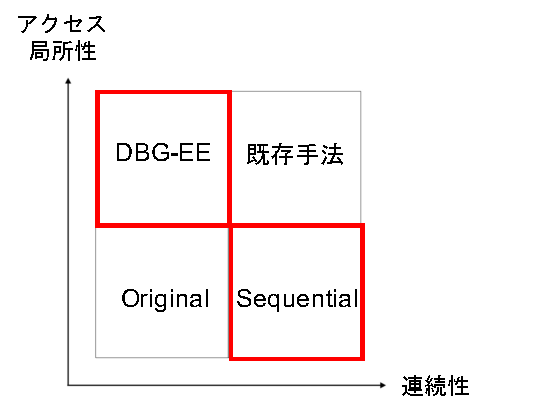
\includegraphics[width=\linewidth]{./figure/research_position.pdf}
  \caption{本研究の位置付け}
  \label{research_position}
\end{figure}
図\ref{research_position}に本研究の位置付けを示す.既存手法では全グラフが手元にあり,
グラフの全体構造が把握可能という前提のもと,演算時のアクセス局所性のみを考慮している.
しかし,自律分散グラフ管理環境においてグラフの取得完了まで全グラフが手元にない状況では,アクセス局所性と ID の連続性の双方を考慮する必要がある.
既存手法では連続性とアクセス局所性の双方が実現されているが,取得完了を待つ必要があるという点で空間・時間コストが発生する.
本研究で提案する Sequential と DBG-EE はそれぞれ ID の連続性と演算時のアクセス局所性を意識した手法となっている.

\section{本論文の構成}
第1章では自律分散グラフ管理形態の概要とノード ID を適切に再配置する必要性を明示した.
そして,空間・時間コストを削減するためにグラフを取得しながらノード ID を再配置する手法として ID の連続性と演算時のアクセス局所性をそれぞれ意識した Sequential と DBG-EE を提案した.
第2章ではグラフ演算におけるノード ID とメモリアクセスの関係及び再配置に伴う ID の連続性とアクセス局所性の重要性について述べる.
第3章では本論文の関連研究について述べる.
第4章では提案手法である Sequential と DDB-EE について述べる.
第5章では提案手法の効果及びグラフ取得の完了を待たない事による空間・時間コストの変化に関して評価を行う.
最後に第6章では本論文における結論と今後の課題について述べる.